\chapter{Introducao} \label{ch:intro}

	O ensino de Engenharia no Brasil se inicia formalmente em 1792, com a criação da Real Academia de Artilharia, Fortificação e Desenho, na cidade do Rio de Janeiro. Esta foi precursora da Escola Politécnica da Universidade Federal do Rio de Janeiro (Poli\abbrev{Poli}{Escola Politécnica}/UFRJ\abbrev{UFRJ}{Universidade Federal do Rio de Janeiro}) e também do Instituto Militar de Engenharia \cite{surgimento_engenharia_brasil}.\\
	
	%Apesar desta instituição ter sido pioneira na América Latina, o Brasil hoje apresenta uma proporção de engenheiros formados relativamente baixa em relação ao total de profissionais egressos das Instituições de Ensino Superior, quando comparado com outros países índice de desenvolvimento humano semelhante \cite{evolucao-formacao-engenheiros-ipea}.\\
	
	A regulamentação nacional da profissão de Engenheiro se dá em 1933, com a criação do Conselho Federal de Engenharia e Arquitetura e dos respectivos Conselhos Regionais, em resposta ao surgimento de outras unidades de ensino através do país e da necessidade de proteger o mercado de profissionais leigos ou inabilitados \cite{historia-confea}.\\
	
	\begin{figure}[h!]
		\centering
		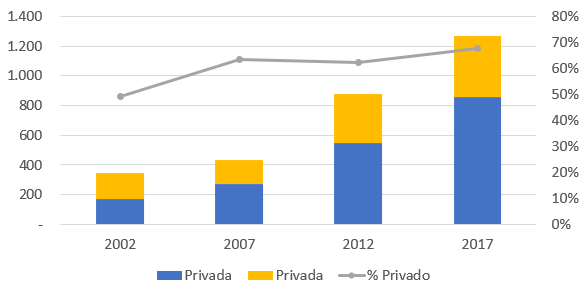
\includegraphics[width=0.8\linewidth]{Figuras/evolucao_cursos_engenharias}
		\caption[Evolução da quantidade de cursos de engenharia elétrica, eletrônica e afins]{Evolução da quantidade de cursos de engenharia elétrica, eletrônica e afins e a respectiva relação entre instituições públicas e privadas \cite{censo_educacao_superior}}
		\label{fig:evolucaocursosengenharias}
	\end{figure}
	
	Nas últimas décadas o número de instituições de ensino e de cursos de engenharia reconhecidos pelo Ministério da Educação vêm apresentando crescimento quantitativo notável, conforme evidenciado pela figura \ref{fig:evolucaocursosengenharias}, que mostra a evolução na quantidade de cursos de engenharia elétrica, eletrônica e afins em Instituições de Ensino Superior (IES\abbrev{IES}{Instituição de Ensino Superior}) públicas e privadas.\\
	
	\begin{figure}[h!]
		\centering
		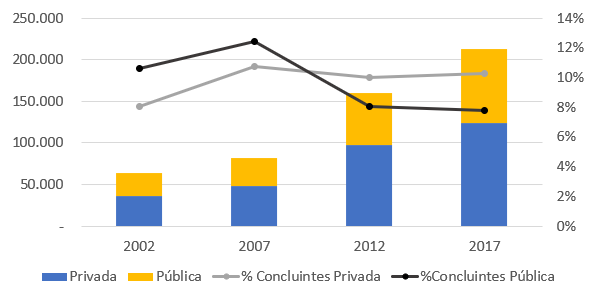
\includegraphics[width=0.8\linewidth]{Figuras/evolucao_matriculados_concluintes}
		\caption[Evolução de matriculados em cursos de engenharia elétrica, eletrônica e afins]{Evolução da quantidade de estudantes matriculados em cursos de engenharia elétrica, eletrônica e afins e a proporção de concluintes sobre o total, em instituições públicas e privadas \cite{censo_educacao_superior}}
		\label{fig:evolucaomatriculadosconcluintes}
	\end{figure}
	
	A figura \ref{fig:evolucaomatriculadosconcluintes} mostra e evolução do volume de estudantes matriculados em cursos de engenharia elétrica, eletrônica e afins e a razão entre a quantidade de concluintes e total de matriculados, considerando IES públicas e privadas. Observamos não apenas uma diminuição da representatividade de IES públicas sobre o total, mas uma diminuição no percentual de estudantes concluintes advindos destas instituições.\\
	
	Além disto, os cursos de engenharia elétrica, eletrônica e afins são os que apresentam maiores valores de multiplicador de emprego \cite{demanda_engenheiros}, isto é, são cursos que tem maior capacidade de serem demandados pelo mercado, especialmente no setor de máquinas, aparelhos e materiais elétricos.
	
	\section{Motivação}
	
		Considerando todos estas tendências, observamos uma relação de oferta e demanda cada vez mais crítica para estes cursos. Paralelamente, cada vez mais levanta-se o debate sobre como a produção de ciência e tecnologia é de extrema relevância não apenas para o desenvolvimento socioeconômico, mas para a soberania nacional como um todo.\\
		
		Neste contexto, é bastante estratégico que seja feita uma reflexão sobre o modelo adotado para construção de conhecimento necessário à formação das próximas gerações de engenheiros, para garantir que estudantes tenham uma formação cada vez mais instigadora e completa. Esta análise se torna ainda mais importante quando se considerando a realidade das IES públicas, já que estas seriam polos para produção de conhecimento voltado para o transformação das sociedades em que se inserem.\\
		
		Neste sentido, uma das primeiras reflexões que podem ser feitas é a respeito das metodologias de ensino utilizadas, suas limitações, potencialidades e de que forma elas podem ser utilizadas para potencializar o processo de aprendizagem.\\
		
		Uma das alternativas de metodologia com grande potencial é a Aprendizagem Baseada em Problemas (APB\abbrev{APB}{Aprendizagem Baseada em Problemas}) - \textit{Problem Based Learning}, em inglês - cuja aplicação já foi estudada em uma disciplina de Engenharia Elétrica no Brasil, apresentando boa aceitação por parte dos estudantes \cite{students_evaluate_pbl}.
		
	% \section{Objetivos}
	
	\section{Objetivo}

		Este projeto tem por objetivo fazer uma análise das formas como engenheiros aprendem, das metodologias que podem ser aplicadas para otimizar este processo e desenvolver um modelo de como elas podem ser aplicadas no curso de Engenharia Elétrica da UFRJ.\\
		
		Para isso, nos focaremos no desenvolvimento de um modelo de APB na disciplina de Máquinas Elétricas I que é uma das disciplinas obrigatórias do Ciclo Profissional. A proposta é que este modelo seja estruturado de forma que possa ser replicado em outras das matérias do curso.
	
	\section{Estrutura do Trabalho}
	
		Este trabalho divide-se nos seguintes capítulos:\\
		
		O \textbf{Capítulo \ref{ch:revisao_ensino}} apresenta uma revisão dos tipos de metodologia de ensino, com enfoque nas aplicações dentro das Engenharias, em particular a APB.
		
		O \textbf{Capítulo \ref{ch:revisao_curso}} faz um levantamento das disciplinas do curso e seu conteúdo, em especial da matéria selecionada para este projeto.
		
		O \textbf{Capítulo \ref{ch:metodo}} mostra o método aplicado para desenvolvimento da proposta de implementação da metodologia.
		
		O \textbf{Capítulo \ref{ch:conclusoes}} apresenta as conclusões e as propostas de projetos futuros.